
%(BEGIN_QUESTION)
% Copyright 2011, Tony R. Kuphaldt, released under the Creative Commons Attribution License (v 1.0)
% This means you may do almost anything with this work of mine, so long as you give me proper credit

Suppose you are asked to connect a pair of split-ranged control valves to a single 4-20 mA analog output of a Siemens 353R rack-mounted controller.  The analog output card plugged into the terminal block assembly (shown) is a model IO-8AO, and the channel you are to use is channel 3:

$$\includegraphics[width=15.5cm]{i03374x01.eps}$$

Sketch the necessary tube and wire connections to make both split-range valves function properly, controlled by channel 3 of the Siemens 353R controller.

\vfil 

\underbar{file i03374}
\eject
%(END_QUESTION)





%(BEGIN_ANSWER)

This is a graded question -- no answers or hints given!
 
%(END_ANSWER)





%(BEGIN_NOTES)

The I/P converters must be connected in {\it series} (to as to share the exact same current with each other) with terminals 5 (+) and 6 ($-$) on the AO card.  A good source of information on the terminal assignments is the Siemens 353R controller manual. 

The ATO valve needs air tubed to the bottom of the actuator, while the ATC valve needs air tubed to the top.   This assumes direct-acting valve bodies in each case.

$$\includegraphics[width=15.5cm]{i03374x02.eps}$$

%INDEX% Pictorial circuit review (analog signal wiring from Siemens 353R controller to two valves)

%(END_NOTES)


